% CMS coordinate system and pseudorapidity for Chapter II (fig:cms_coordinates).
% Adapted from https://tikz.net/axis3d_cms/ and https://tikz.net/axis2d_pseudorapidity/
% (Izaak Neutelings, CC BY-SA 4.0).
% Each tikzpicture is one page of the PDF: page 1 is panel (a), page 2 is panel (b).
\documentclass[tikz,border=2pt]{standalone}
\usepackage[T1]{fontenc}
\usepackage{cochineal}
\usepackage[cochineal]{newtxmath}
\usepackage{tikz-3dplot}
\usetikzlibrary{arrows.meta,3d,bending,angles,quotes,fpu}
\usepackage[outline]{contour} % glow around text
\contourlength{0.9pt}

\colorlet{myred}{red!70!black}
\colorlet{mycontourred}{red!55!black!3}
\colorlet{mycontourred2}{red!55!black!6}
\colorlet{mydarkred}{red!40!black}
\colorlet{CMScol}{red!80!black}
\tikzset{>=latex}
\tikzstyle{axis}=[->,thick,line cap=round]
\tikzstyle{detector}=[thick,draw=mydarkred,rotate around z=\ang]
\tikzstyle{beam pipe}=[draw=blue!20!black!50,fill=blue!20!black!10,rotate around z=\ang]
\tikzstyle{detector surface}=[red!60!black!10,opacity=0.5,rotate around z=\ang]
\tikzset{
  eta line/.style={->,black!60!red,thick,line cap=round},
  theta node/.style={black,pos=0.7,fill=white,scale=0.8,inner sep=1.2pt,rounded corners=2pt},
  mysmallarrow/.style={-{Latex[length=3,width=2.5]},draw=black,line width=0.6,
                       angle radius=30,angle eccentricity=1.25}
}

\begin{document}

% (a) CMS DETECTOR AND COORDINATE SYSTEM
\tdplotsetmaincoords{75}{50}
\begin{tikzpicture}[scale=2.0,tdplot_main_coords,rotate around x=90,every node/.style={font=\small}]
  \def\rvec{\L/2/cos(\thetavec)}
  \def\thetavec{18}
  \def\phivec{60}
  \def\L{3.3}    % detector length
  \def\R{0.75}   % detector radius
  \def\l{4.3}    % beam pipe length
  \def\r{0.04}   % beam pipe radius
  \def\rt{0.042} % beam pipe radius + line thickness
  \def\xmax{1}
  \def\ymax{1}
  \def\zmin{-\l/2-0.2}
  \def\zmax{\l/2+0.3}
  \def\w{0.3}
  \coordinate (O) at (0,0,0);
  \coordinate (Z) at (0,0,\L/2);
  \tdplotsetcoord{O'}{0.022}{\thetavec}{\phivec}
  \tdplotsetcoord{O''}{0.018}{90}{\phivec}
  \tdplotsetcoord{P}{\rvec}{\thetavec}{\phivec}

  % cylinder, behind
  \def\ang{18}
  \fill[top color=red!50!black!4,bottom color=red!60!black!2,rotate around z=\ang]
    (0,\R,\L/2) --++ (0,0,-\L) arc(90:270:\R) --++ (0,0,\L) arc(270:90:\R) -- cycle;
  \fill[detector surface] (0,0,\L/2) --++ (0,\R,0) arc(90:270:\R) -- cycle;
  \fill[detector surface] (0,0,-\L/2) --++ (0,\R,0) arc(90:270:\R) -- cycle;
  \tdplotdrawarc[detector]{(0,0,\L/2)}{\R}{0}{360}{}{}
  \tdplotdrawarc[detector,thin]{(0,0,-\L/2)}{\R}{0}{360}{}{}
  \draw[detector,thin] (90:\R) arc (90:270:\R);
  \draw[detector,very thin] (90:\R) arc (90:90-\ang:\R);
  \draw[detector] (0,0,-\L/2)++(90:\R) --++ (0,0,\L);
  \draw[detector] (0,0,-\L/2)++(-90:\R) --++ (0,0,\L);

  % beam pipe
  \tdplotdrawarc[beam pipe]{(0,0,\l/2)}{\r}{0}{360}{}{}
  \draw[beam pipe]
    (0,\r,-\l/2) -- (0,\r,-0.2*\l) -- (90:0.5*\r)
    -- (0,\r,0.2*\l) -- (0,\r,0.5*\l) arc(90:-90:\r)
    -- (0,-\r,0.2*\l) -- (-90:0.5*\r) --
    (0,-\r,-0.2*\l) -- (0,-\r,-\l/2) arc(-90:90:\r);
  \draw[beam pipe] (0,0,\l/2) circle(\r);

  % axes
  \draw[axis,-] (0,0,\zmin) -- (0,0,0);
  \fill[CMScol] (O) circle(0.5pt) node[right=1,below=1] {IP};
  \draw[axis] (0,0,0.020) -- (0,0,\zmax) node[right=3,below=1]{$z$};
  \draw[axis] (0,0.019,0) -- (0,\ymax,0) node[below left]{$y$};
  \draw[dashed,myred] (O'')  -- (Pxy);
  \draw[axis] (0.022,0,0) -- (\xmax,0,0) node[below=1,right=-2]{$x$};

  % pseudorapidity labels
  \node[mydarkred,above] at (0,\ymax,0) {$\eta=0$};
  \node[mydarkred,above=3] at (0,\R,0.3*\L) {$\eta>0$};
  \node[mydarkred,above=3] at (0,\R,-0.2*\L) {$\eta<0$};
  \node[mydarkred,below=1,left] at (0,0,\zmax) {$\eta=+\infty$};
  \node[mydarkred,above=1,right] at (0,0,\zmin) {$\eta=-\infty$};

  % momentum and its transverse projection
  \draw[dashed,myred] (Px) -- (Pxy);
  \draw[->,red,line cap=round] (O'') -- (Pxy) node[anchor=170,inner sep=2pt] {$\vec{p}_T$};
  \draw[dashed,myred,line join=round] (Py) -- (Pxy) -- (P);
  \draw[->,red,line cap=round] (O') -- (P);

  % cylinder, front
  \draw[beam pipe,fill=none] (0,\r,-\l/2) arc(90:-90:\r);
  \fill[detector surface]
    (0,\rt,\L/2) --++ (0,\R-\rt,0) arc(90:-90:\R) --++ (0,\R-\rt,0) arc(-90:90:\rt);
  \fill[detector surface]
    (0,\rt,-\L/2) --++ (0,\R-\rt,0) arc(90:-90:\R) --++ (0,\R-\rt,0) arc(-90:90:\rt);
  \tdplotdrawarc[detector]{(0,0,\L/2)}{\R}{-90}{90}{}{}
  \tdplotdrawarc[detector]{(0,0,-\L/2)}{\R}{-90}{90}{}{}
  \draw[beam pipe,fill=none] (0,\r,\l/2) arc(90:-90:\r);
  \draw[detector,very thin] (90-\ang:\R) arc (90-\ang:-90:\R);
  \node[red,anchor=-30,inner sep=2pt] at (P) {$\vec{p}$};
  \draw[dashed,myred] (Pz) -- (P);

  % angles
  \tdplotdrawarc[thick,mycontourred]{(O)}{0.2}{4}{0.7*\phivec}{}{}
  \tdplotdrawarc[draw=none,opacity=0.9]{(O)}{0.2}{0}{\phivec}
    {anchor=-150,inner sep=1pt}{\contour{mycontourred}{$\phi$}}
  \tdplotdrawarc[->]{(O)}{0.2}{0}{\phivec}
    {anchor=-150,inner sep=1pt}{$\phi$}
  \tdplotdrawarc[->,rotate around z=\phivec-90,rotate around y=-90]
    {(O)}{0.88}{0}{\thetavec}
    {anchor=-20,inner sep=2pt}{$\theta$}
  \tdplotdrawarc[thick,red!58!black!4,rotate around z=\phivec-90,rotate around y=-90]
    {(O)}{0.3}{88}{0.5*(90+\thetavec)}{}{}
  \tdplotdrawarc[-{>[flex'=1]},rotate around z=\phivec-90,rotate around y=-90,line cap=round]
    {(O)}{0.3}{90}{\thetavec}
    {anchor=-40,inner sep=1pt}{$\eta$}
  \draw[mydarkred] (0,0,\L/2) --++ (\R,0,0);
  \tdplotdrawarc[thick,mycontourred2]{(Z)}{0.2}{4}{0.7*\phivec}{}{}
  \tdplotdrawarc[draw=none,opacity=0.9]{(Z)}{0.2}{0}{\phivec}
    {anchor=-150,inner sep=1pt}{\contour{mycontourred2}{$\phi$}}
  \tdplotdrawarc[->]{(Z)}{0.2}{0}{\phivec}
    {anchor=-150,inner sep=1pt}{$\phi$}

  % direction of the centre of the LHC (x axis)
  \draw[->,thick,orange!30!black] (1.4*\w,-\R,-0.1*\L) --++ (2*\w,0,0)
    node[below=1,right,scale=0.85,align=center] {center of\\[-1pt]the LHC};
\end{tikzpicture}

% (b) PSEUDORAPIDITY AS A FUNCTION OF THE POLAR ANGLE
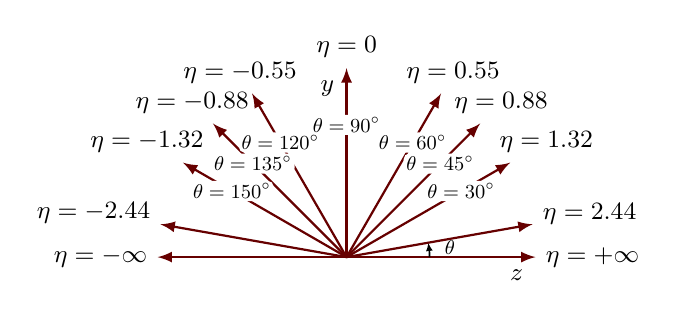
\begin{tikzpicture}[scale=2.0,every node/.style={font=\small}]
  \pgfkeys{/pgf/fpu/output format=fixed,/pgf/number format/precision=2}
  \def\R{1.2}
  \coordinate (O) at (0,0);
  \node[below left=1] at (0,\R) {$y$};
  \node[below left=1] at (\R,0) {$z$};
  \foreach \t in {180,170,150,135,120,90,60,45,30,10,0}{
    \ifnum \t = 0
      \def\e{+\infty}
    \else \ifnum \t = 180
      \def\e{-\infty}
    \else
      \pgfkeys{/pgf/fpu=true}
      \pgfmathparse{-ln(tan(\t/2))}
      \pgfkeys{/pgf/fpu=false}
      \pgfmathroundtozerofill{\pgfmathresult}
      \pgfmathsetmacro\e{\t==90?0:\pgfmathresult}
    \fi \fi
    \draw[eta line] (O) -- (\t:\R) coordinate(P\t) node[anchor=180+\t,black] {$\eta=\e$};
  }
  % polar angle only on the lines far enough from the beam, to avoid overlaps
  \foreach \t in {150,135,120,90,60,45,30}{
    \path (O) -- (\t:\R) node[theta node] {$\theta=\t^\circ$};
  }
  \draw pic["$\theta$"scale=0.8,mysmallarrow] {angle = P0--O--P10};
\end{tikzpicture}

\end{document}
